\documentclass{beamer}
\usepackage{HECbeamer}
% \usepackage{pgfpages}
% \pgfpagesuselayout{4 on 1}[letterpaper, landscape, border shrink=5mm]
\title[\color{white}{MATH 60604A \S~6a - Group effects}]{\texorpdfstring{MATH 60604A \\Statistical modelling \\ \S~6a - Group effects}{MATH 60604A \\Statistical modelling \\ \S~6a - Group effects}}
\author{Léo Belzile}
\institute{HEC Montréal\\
Department of Decision Sciences}
\date{} 

\begin{document}
\frame{\titlepage}
% \begin{frame}
% \frametitle{Overview of course material}
% \begin{center}
% \includegraphics[scale=0.35]{Figures/fig6.png}
% \end{center}
% \end{frame}
% \section{Inclusion of group effect for the mean}
\begin{frame}
 \frametitle{Inclusion of group effects}
 \bi 
 \item So far, we have only accounted for group structure by modelling the within-group correlation.
 \item We may also want to include a \alert{group effect} in the mean model, i.e., a different intercept for each group.
 \item This is done by adding the categorical group variable \texttt{g} as explanatory variable in the mean model, which translates into $m-1$ indicator variables $\I{\code{g}=i}$ for $i=1, \ldots, m-1$ if there are $m$ groups. 
 \item Suppose that we only include the categorical variable \code{g} representing groups,
 \[ Y_{ij}= \beta_0 + \sum_{i=1}^{m-1} \beta_i\I{\code{g}=i} + \eps_{ij},\]
 \bi \item for the baseline (group $m$), the intercept is $\beta_0$,
 \item the group effect for $\code{g}=i$ is $\beta_i$ $(i=1, \ldots, m-1)$, and the overall group-specific ``intercept'' is $\beta_0+ \beta_i$.
 \ei
 \ei
 
 \end{frame}
 
\begin{frame}
\frametitle{Linear model with a group effect for the \texttt{revenge} data}
We consider a regression model for \texttt{revenge} with a group effect to illustrate the challenges.
\bi
\item The idea here is to model the fact that desire for revenge can vary between subjects.
\item In the current example, there are only five observations per person to estimate the group effect.
% \item To do this, we can use a model that includes a different parameter for each person. 
\item The model will ignore the within-person correlation for now.
% \item First we'll see how to fit a model with a group (or subject) effect without correlation.
% \item We will include the correlation in this model later on.
\ei
\end{frame}




\begin{frame}[fragile]
\frametitle{Model with group effects for subject}
\begin{tcolorbox}[colback=white, colframe=hecblue, title=\SASlang{} code to fit a linear model via REML]
\begin{verbatim}
proc mixed data=revenge method=reml; 
class id; 
model revenge = id sex age vc wom t / solution; 
run;
\end{verbatim}
\end{tcolorbox}
{\footnotesize In addition to the categorical variable \code{id}, the model includes the same explanatory variables as before. Each person has his/her own ``intercept'' parameter (\texttt{id=80} is the baseline category). 


}
\end{frame}

 \begin{frame}
\frametitle{Estimates of fixed effects}
\begin{center}
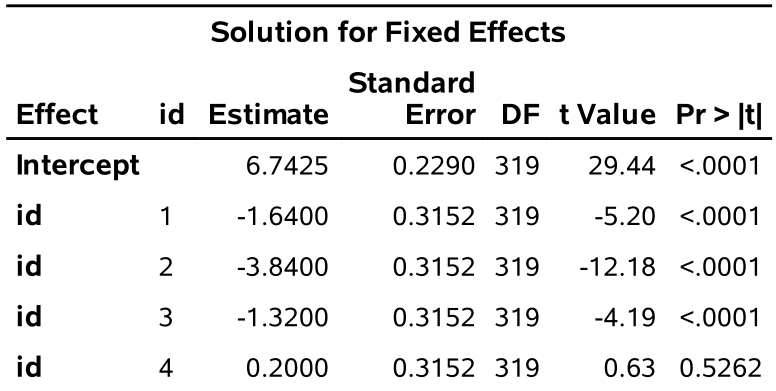
\includegraphics[width = 0.6\linewidth]{img/c6/slides7-e01}
\begin{align*}
\vdots      \end{align*}



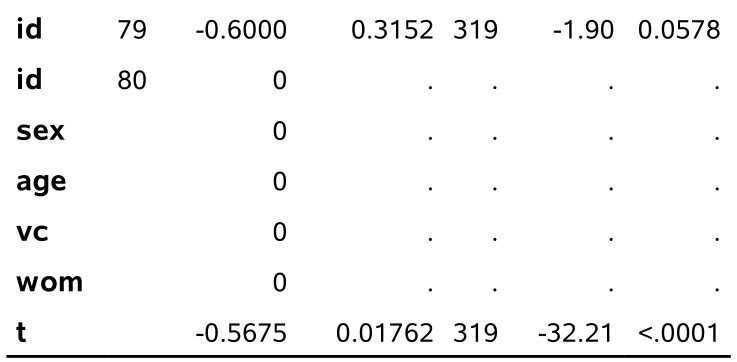
\includegraphics[width = 0.6\linewidth]{img/c6/slides7-e02}
\end{center}

\end{frame}

%  \begin{frame}
% \frametitle{\SASlang{} output}
% \textbf{Estimates of fixed effects (continued)}
% \begin{center}
% \includegraphics[scale=0.35]{Figures/long53.pdf}
% \end{center}
% \end{frame}

 \begin{frame}
\frametitle{Parameter significance}
\begin{center}
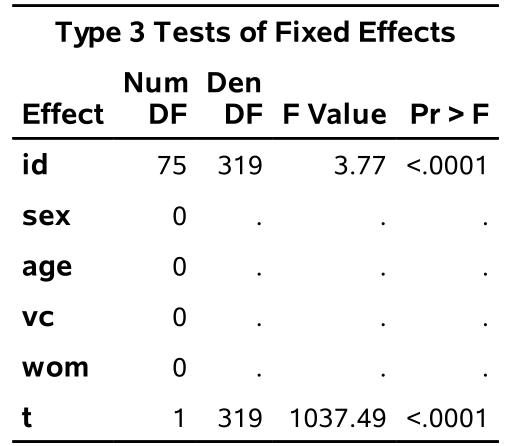
\includegraphics[width=0.4\linewidth]{img/c6/slides7-e03}
\end{center}
{\footnotesize 


There are \textbf{no} parameters estimates or tests for the variables \code{sex}, \code{age}, \code{vc} or \code{wom}, but there is for the time variable \code{t}. 
Because some covariates are fixed over time, their effect are not uniquely estimable (perfect collinearity). If we remove \code{id} from the model, we can however estimate their effects (hence $75$ \code{df} rather than $79$ in the $F$-table).

}
\end{frame}


\begin{frame}[fragile]
\frametitle{Collinearity}
\bi
\item  Once we've included a fixed effect for each person, \alert{it is impossible to include any variable that does not vary in time for a single person}. 
\item The variables \code{sex}, \code{age}, \code{vc} and \code{wom} are fixed in time for each person (\code{vc} and \code{wom} were only measured once, at time 1). 
\item These variables are already implicitly included in the individual effect. There is \alert{perfect collinearity} between a variable fixed in time, and the \code{id} variable. 
\item This means that we can perfectly predict the value of \code{sex} (and the three others) by only looking at the \code{id} variable. 
\item Therefore, we cannot have a fixed effect for each individual while simultaneously including variables that are fixed in time for each subject.
\ei
\end{frame}
 \begin{frame}
 \frametitle{Challenges arising from the inclusion of a group effect}
 
 \bi 
 \item Group is a categorical variable: we need enough observations in each group to reliably estimate the group effects.
 \item If the number of groups $m$ is large relative to the overall sample size, there may also be too many parameters in the model. 
 \item We cannot estimate the effect of variables that do not vary within group if we add group effects.
  \ei
\end{frame}


%  \begin{frame}
% \frametitle{\SASlang{} output}
% \textbf{Estimates of fixed effects (continued)}
% \begin{center}
% \includegraphics[scale=0.45]{Figures/long55.pdf}
% \end{center}
% \bi
% \item Each person has his/her own parameter (except for id=80, the reference category). 
% \item There are \alert{no} parameters or tests for the variables \code{sex}, \code{age}, \code{vc} or \code{wom}. But there is for the time variable \code{t}. 
% \item \textbf{\alert{What happened? }}
% \ei
% 
% \end{frame}

% 
% \begin{frame}[fragile]
% \frametitle{Model with fixed effects for subject}
% \bi
% \item  More generally, with correlated observations within groups, if we add a fixed effect for each group, \alert{we cannot include other variables that do not vary within group}.
% \ei
% \end{frame}

\begin{frame}[fragile]
\frametitle{Model with group effect and correlation structure}
The model fitted next includes only \code{id} and the time variable \texttt{t} as explanatory variables in the mean model, but we specify in addition an $\mathsf{AR}(1)$ correlation structure within-individual for the errors $\bs{\eps}$.

\begin{tcolorbox}[colback=white, colframe=hecblue, title=\SASlang{} code to include a group effect with $\mathsf{AR}(1)$ correlation]
\begin{verbatim}
proc mixed data=revenge method=reml; 
class id tcat; 
model revenge = id t / solution; 
repeated tcat / subject=id type=ar(1); 
run;
\end{verbatim}
\end{tcolorbox}
{\footnotesize  The effect of the $\mathsf{AR}(1)$ correlation parameter is significant (likelihood ratio test statistic of $21.68$, negligible $p$-value under $\chi^2_1$). The estimate of the time effect is $-0.5684$, very close to that we got in the model including \code{sex}, \code{age}, \code{vc} and \code{wom}, and the  $\mathsf{AR}(1)$ structure model in the previous chapter. 

}
\end{frame}
% 
% \begin{frame}
% \frametitle{\SASlang{} output}
% \textbf{Estimates of covariance/correlation parameters}
% \begin{center}
% \includegraphics[scale=0.4]{Figures/long56.pdf}
% \includegraphics[scale=0.4]{Figures/long57.pdf}
% \end{center}
% \bi
% \item 
% \ei
% \end{frame}

% \begin{frame}
% \frametitle{Estimates of fixed effects}
% \begin{center}
% \includegraphics[scale=0.35]{Figures/long58.pdf}
% \end{center}
% \end{frame}
% 
% \begin{frame}
% \frametitle{Estimates of fixed effects (continued)}
% \begin{center}
% \includegraphics[scale=0.32]{Figures/long59.pdf}
% \end{center}
% \end{frame}
% 
% \begin{frame}
% \frametitle{Estimates of fixed effects (continued)}
% \begin{center}
% \includegraphics[scale=0.32]{Figures/long60.pdf}
% \end{center}
% \end{frame}
% 
% \begin{frame}
% \frametitle{Estimates of fixed effects (continued)}
% \begin{center}
% \includegraphics[scale=0.35]{Figures/long61.pdf}
% \end{center}
% \bi
% \item Estimates of parameters for time $23$--$78$ are omitted, but they are non-zero.
% \item The global effect of \code{id} is significant, as well as the effect for time. 
% \item 
% \item In that model, the effect of time was estimated as $-0.5686$.
% \ei
% \end{frame}

\begin{frame}[fragile]
\frametitle{Remark on model comparison}
\bi
\item We have to be careful \alert{not to use} the \ensuremath{\mathsf{AIC}}{} and \ensuremath{\mathsf{BIC}}{} reported in the output to compare this model to the earlier one including \code{sex}, \code{age}, \code{vc} and \code{wom}, since we used the REML estimation method (the default). 
\item \ensuremath{\mathsf{AIC}}{} and \ensuremath{\mathsf{BIC}}{} obtained through REML, are \textbf{not comparable} if the ``mean'' parts of the models (fixed effects) are not the same. 
\item If we want to compare these models, we must use the maximum likelihood estimator (option \texttt{method=ml} when calling \code{proc mixed}). 
\ei
 \begin{center}
  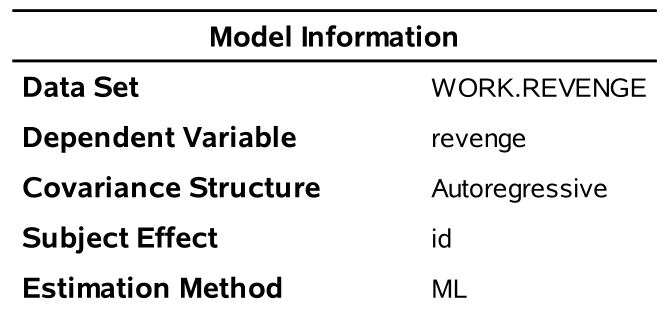
\includegraphics[width = 0.5\linewidth]{img/c6/slides7-e05}
 \end{center}
   
\end{frame}


\begin{frame}[fragile]
\frametitle{Remark on model comparison}
We fit both models with an $\mathsf{AR}(1)$ structure for the errors using maximum likelihood.
\begin{center}
\begin{tabular}{c c c r}
\toprule 
\textbf{Model} & \textbf{AIC} & \textbf{BIC} & $\hat{\rho}$ ($p$-value)\\ \midrule 
\code{sex}, \code{age}, \code{vc}, \code{wom}, \code{t} & 666.1 & \alert{685.1}  & $0.48$ ($10^{-20}$) \\
\code{id}, \code{t} & \alert{653.4} & 851.1 & $-0.013$ ($0.83$)\\ \bottomrule
\end{tabular}
\end{center}
\bi
\item The preferred model according to $\mathsf{AIC}$ includes \code{id}, but $\mathsf{AIC}$ tends to select complicated models.
\item The preferred model according to $\mathsf{BIC}$ includes \code{sex}, \code{age}, \code{vc} and \code{wom} and throws away the \code{id} variable.
\item Once we include an individual effect for group, the correlation
structure seems to be unnecessary --- the estimated coefficient is even negative, which is counter-intuitive and suggests the model is over-parametrized.
\ei
\end{frame}

\begin{frame}
\frametitle{Remark on model comparison}
\bi
\item The choice of covariates depends on the type of study. If we're interested in studying the effects of one or more of the variables \code{sex}, \code{age}, \code{vc} or \code{wom}, then we don't have any choice: we must choose a model that contains all of them. 
\item If we're only interested in the time effect, then the two models will come to the same conclusion either way.
 \item Often, the optimization routine fails --- we cannot estimate both the $\bs{\beta}$ and the covariance matrix parameters.
\item It is possible to include variables that are fixed within group (within person in our example) \textbf{and} group effects (\code{id} in our example) at the same time by using \alert{random effects}.
\ei
\end{frame}
\end{document}
